

Para realizar las simulaiones se tomaron los datos correspondientes al modelo del pistón de \cite{Electro-hydraulic_actuator}, los cuales se muestran en la Tabla \ref{tab_valoresmodelo}. 


\begin{center}
	\captionof{table}{Valores del Modelo}
	\label{tab_valoresmodelo} 
	\begin{tabular}[t]{clccl}
		$m$ & $24kg$ & & $k_s$ & $1610 N/m$\\
		$b_d$ & $310N/(m/s)$ & & $Ps$ & $1.03e7 pa$\\
		$\Lambda_a$ & $3.26e-4 m^2$ & & $\alpha$ & $1.51e10 N/m^3$\\
		$\beta$ & $1 1/s$ & & $\gamma$ & $7.28e8 g^{0.5}/m^{1.5}s^2$\\
		$M$ & $300-500 N$ & & $a_n$ & $2.4315e5$\\
		$b_n$ & $6.2529e2$ & & $c_n$ & $2.5676e5$
	\end{tabular}
\end{center}

La posición inicial para cada agente es $[0,0.1,0.2,0.3,0.4,0.5]$, el periodo de consensus $T_c=0.5 [s]$, matriz de adyacencia es uan martriz de unos con ceros en la diagonal (fully connected),los valores iniciales de las demás variables de estado para todos los actuadores es $[0,6e6,0,0]$, los valores de carga para cada actuador $[300,300,310,350,590,700]$, los valores de las constantes del controlador son $k_p=1e-2$ y $k_i=1e-6$, el periodo de solución para la planta $T_s=0.1 [s]$, el valor del numerado de la función barrera $b_a=1e-3$ valore de referencia para el consensus $0.7$  y finalmente el tiempo total de la solución es $40 [s]$.


\begin{figure}[!h]
	\centering
	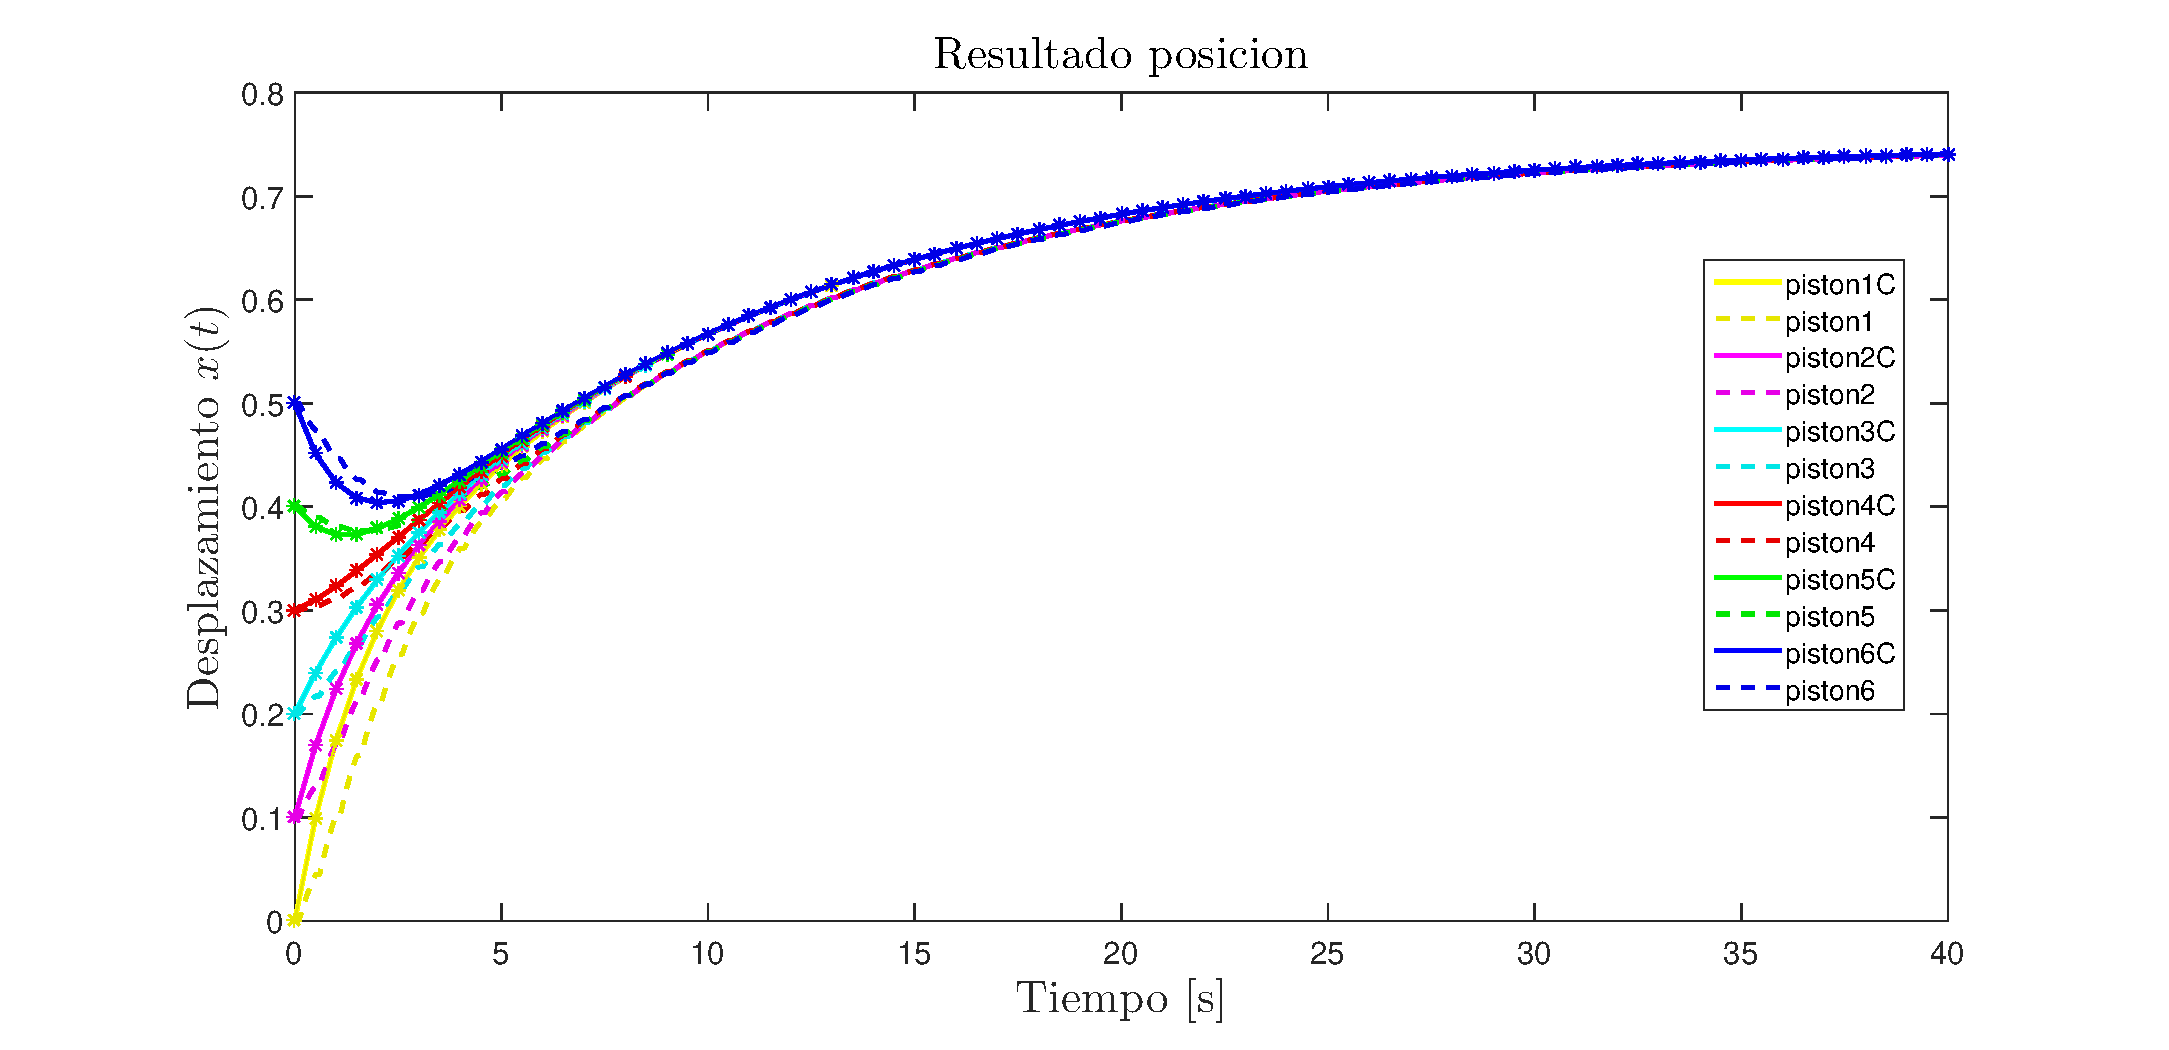
\includegraphics[width=3.9in]{imagenes/consensus_pos.eps}
	\caption{Consensus en tiempo}
	\label{fig_consensus_pos}
\end{figure}
El resultado es como el esperado, se pueden diferenciar dos dinámicas en el resultado de la Figura \ref{fig_consensus_pos}, donde  primero se trata de minimizar las diferencias entre agentes y a medida que se van acercando comienzan a converger en grupo al valor de referencia del consensus, observamos que las posiciones reales (líneas punteadas) siguen con los valores de referencia de manera suave por tanto los periodos para cada sistema son los adecuados.

\begin{figure}[!h]
	\centering
	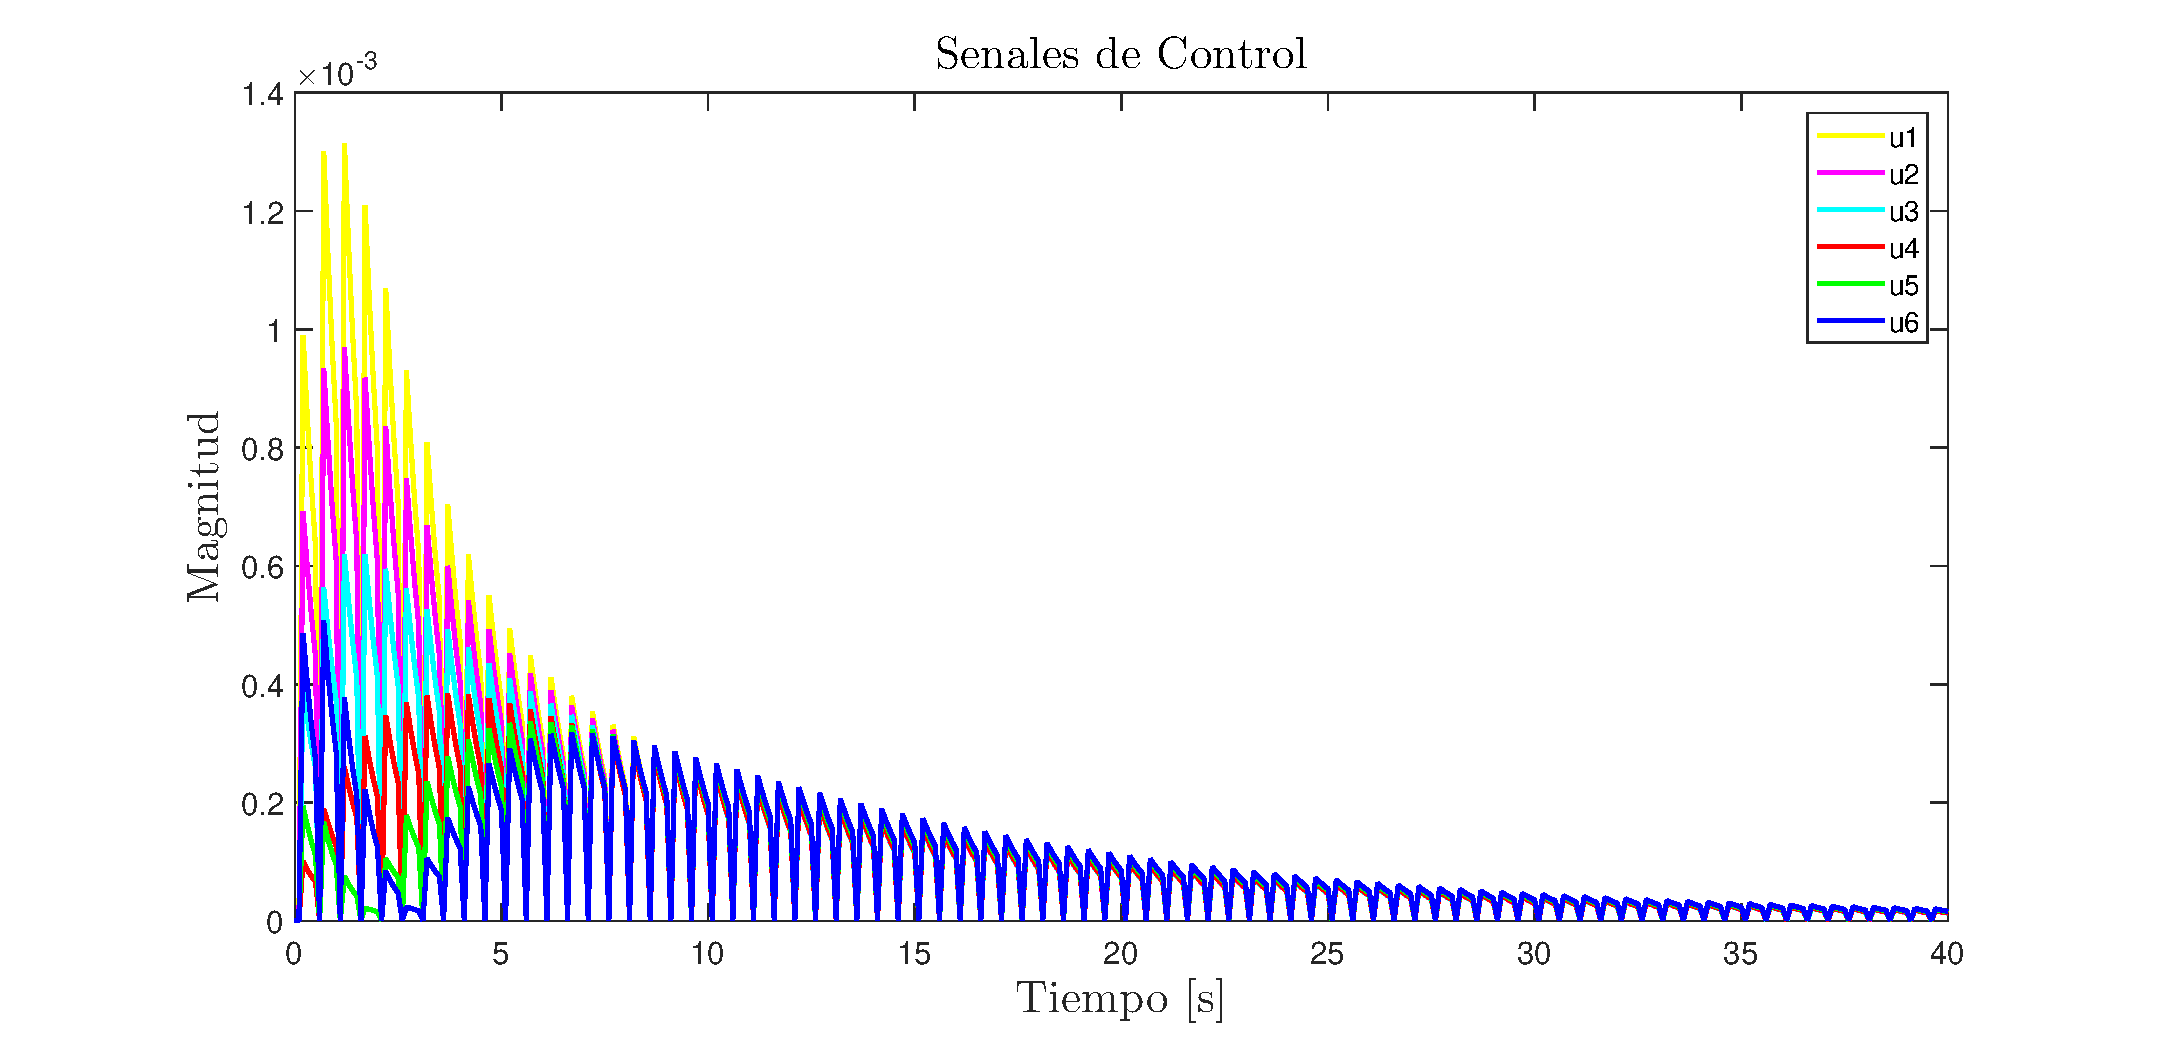
\includegraphics[width=3.9in]{imagenes/senales_conrtrol.eps}
	\caption{Señales de Control en tiempo}
	\label{fig_senales_conrtrol}
\end{figure}

Las señales de control Figura \ref{fig_senales_conrtrol} más altas inicialmente son las de los agentes más lejanos al punto de encuentro. Una vez los agentes confluyen a la misma posición, en su recorrido grupal al valor de referencia, las señales de control son las mismas y van disminuyendo a medida que convergen, el cual es el comportamiento esperado.

\begin{figure}[!h]
	\centering
	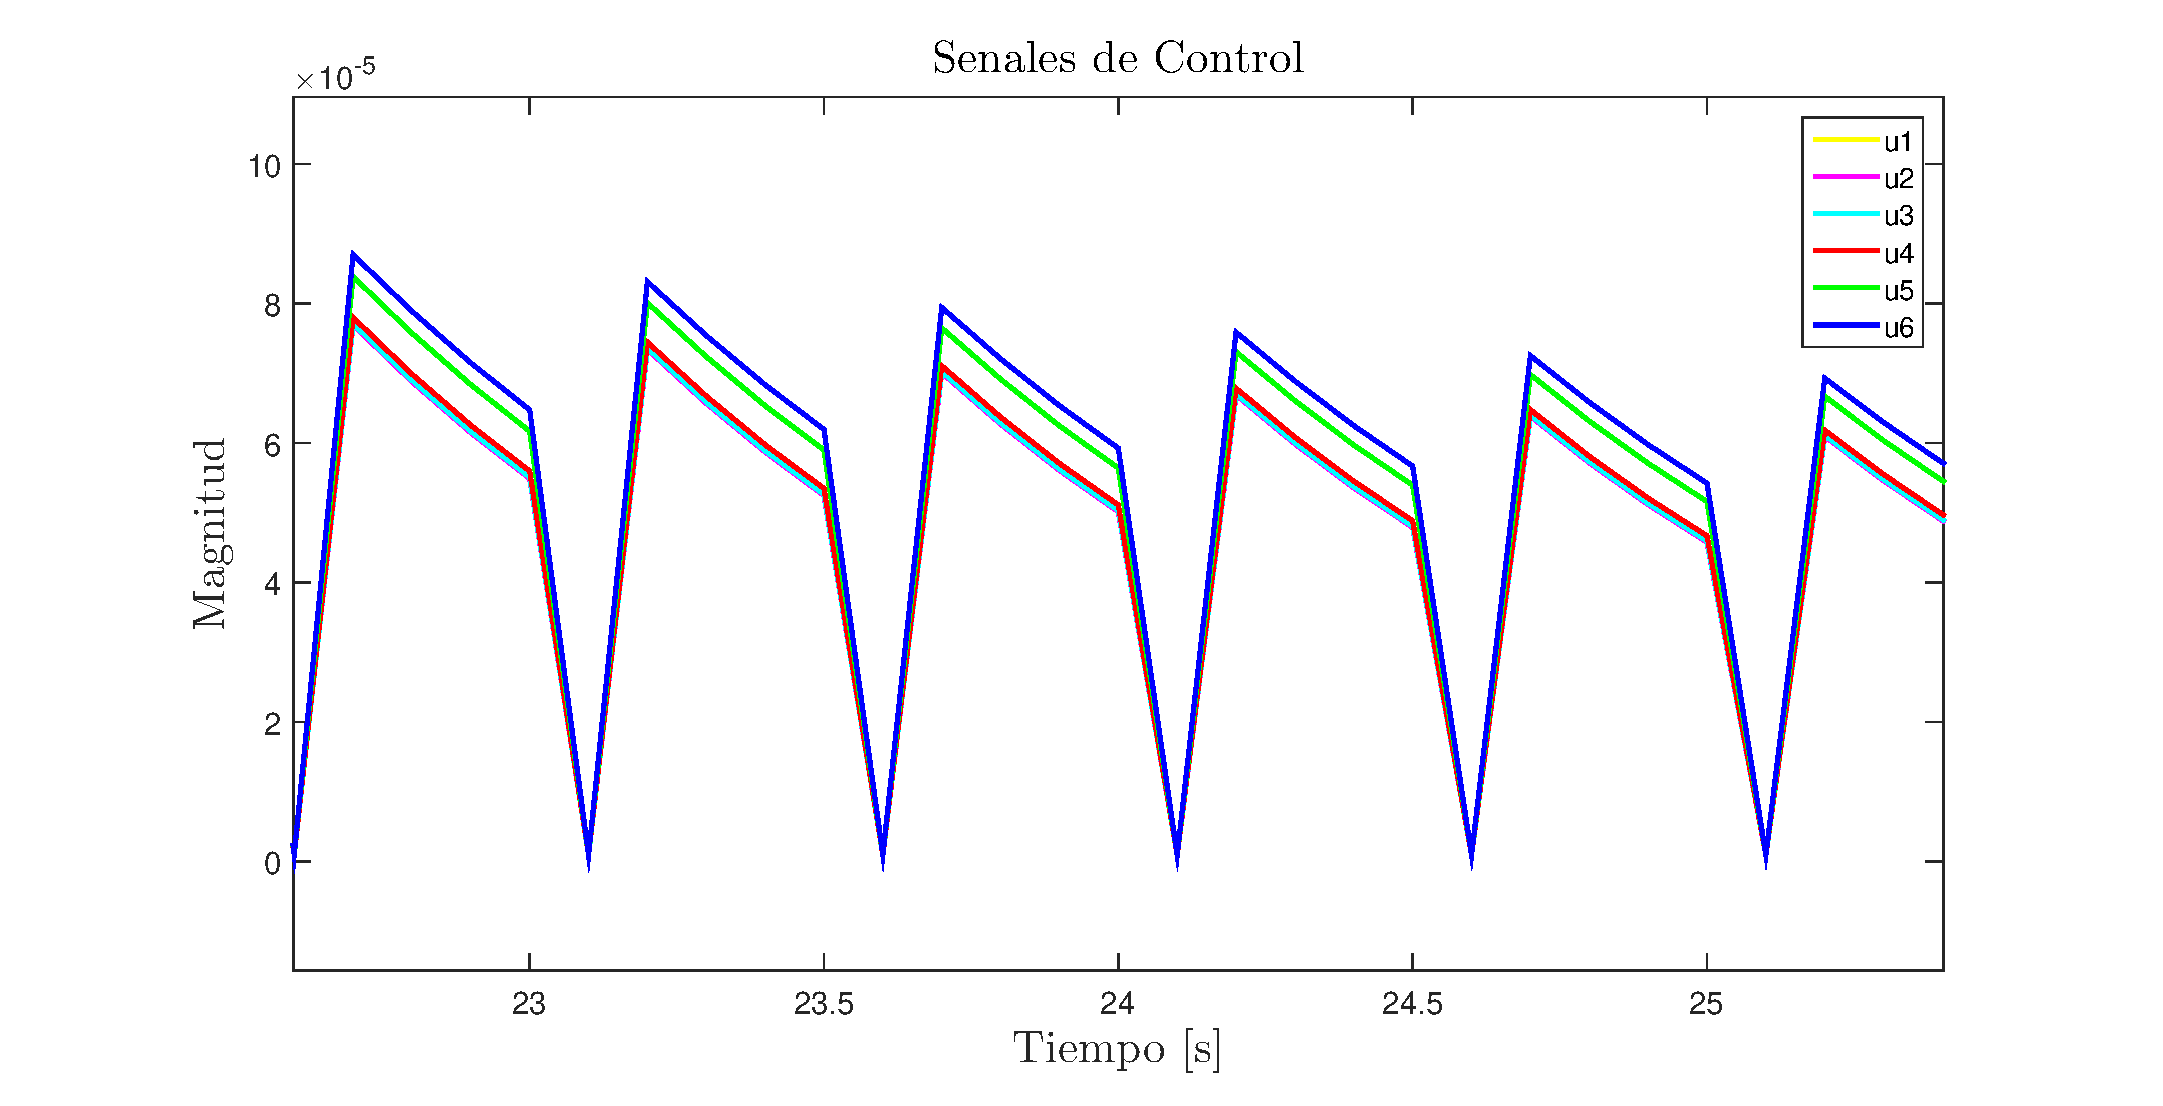
\includegraphics[width=3.9in]{imagenes/senales_conrtrol_zoom.eps}
	\caption{Zoom Señales de Control en tiempo}
	\label{fig_senales_conrtrol_zoom}
\end{figure}
En la Figura \ref{fig_senales_conrtrol_zoom} se evidencian algunas diferencias en las señales de control, esto corresponde a las diferentes caras que tiene cada actuador, vemos que las señales más altas corresponden a los actuadores que tienen más peso sobre ellos, por tanto las dinámicas propias del consensus hacen que se equilibren estas diferencias.

\begin{figure}[!h]
	\centering
	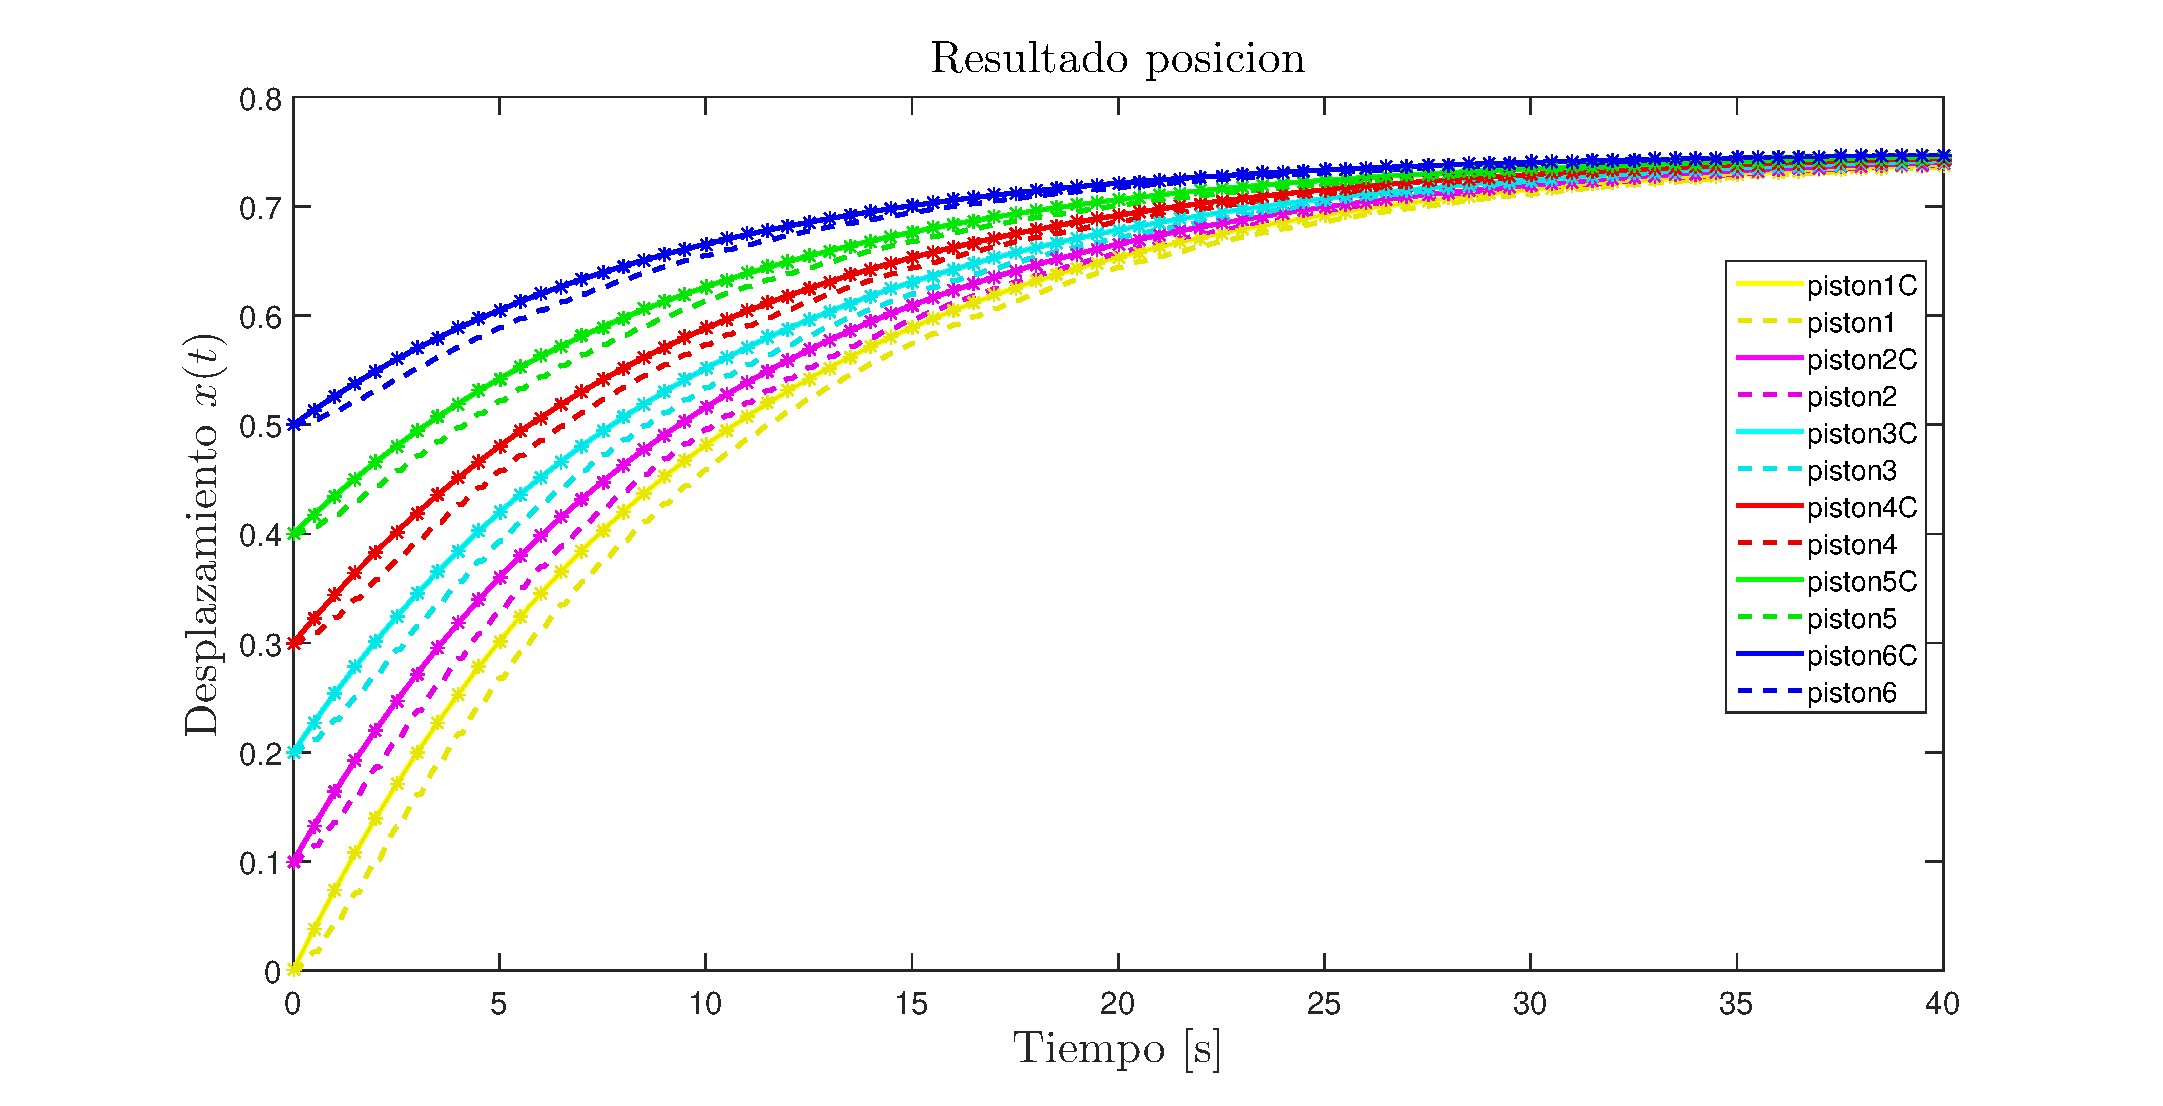
\includegraphics[width=3.9in]{imagenes/consensus_pos_min.eps}
	\caption{Consensus en tiempo para un grafo mínimamente conectado}
	\label{fig_consensus_pos_min}
\end{figure}
En la Figura \ref{fig_consensus_pos_min} se muestra el resultado para el sistema cuando el grafo justo cumple la condición de ser un árbol de alcance directo, es decir los agentes no se conectan entre ellos, sólo se conectan con el líder virtual. El resultado confirma que que se llega a un consensus en el valor de referencia, pero sus dinámicas cambian, solo dependen de la referencia.

\begin{figure}[!h]
	\centering
	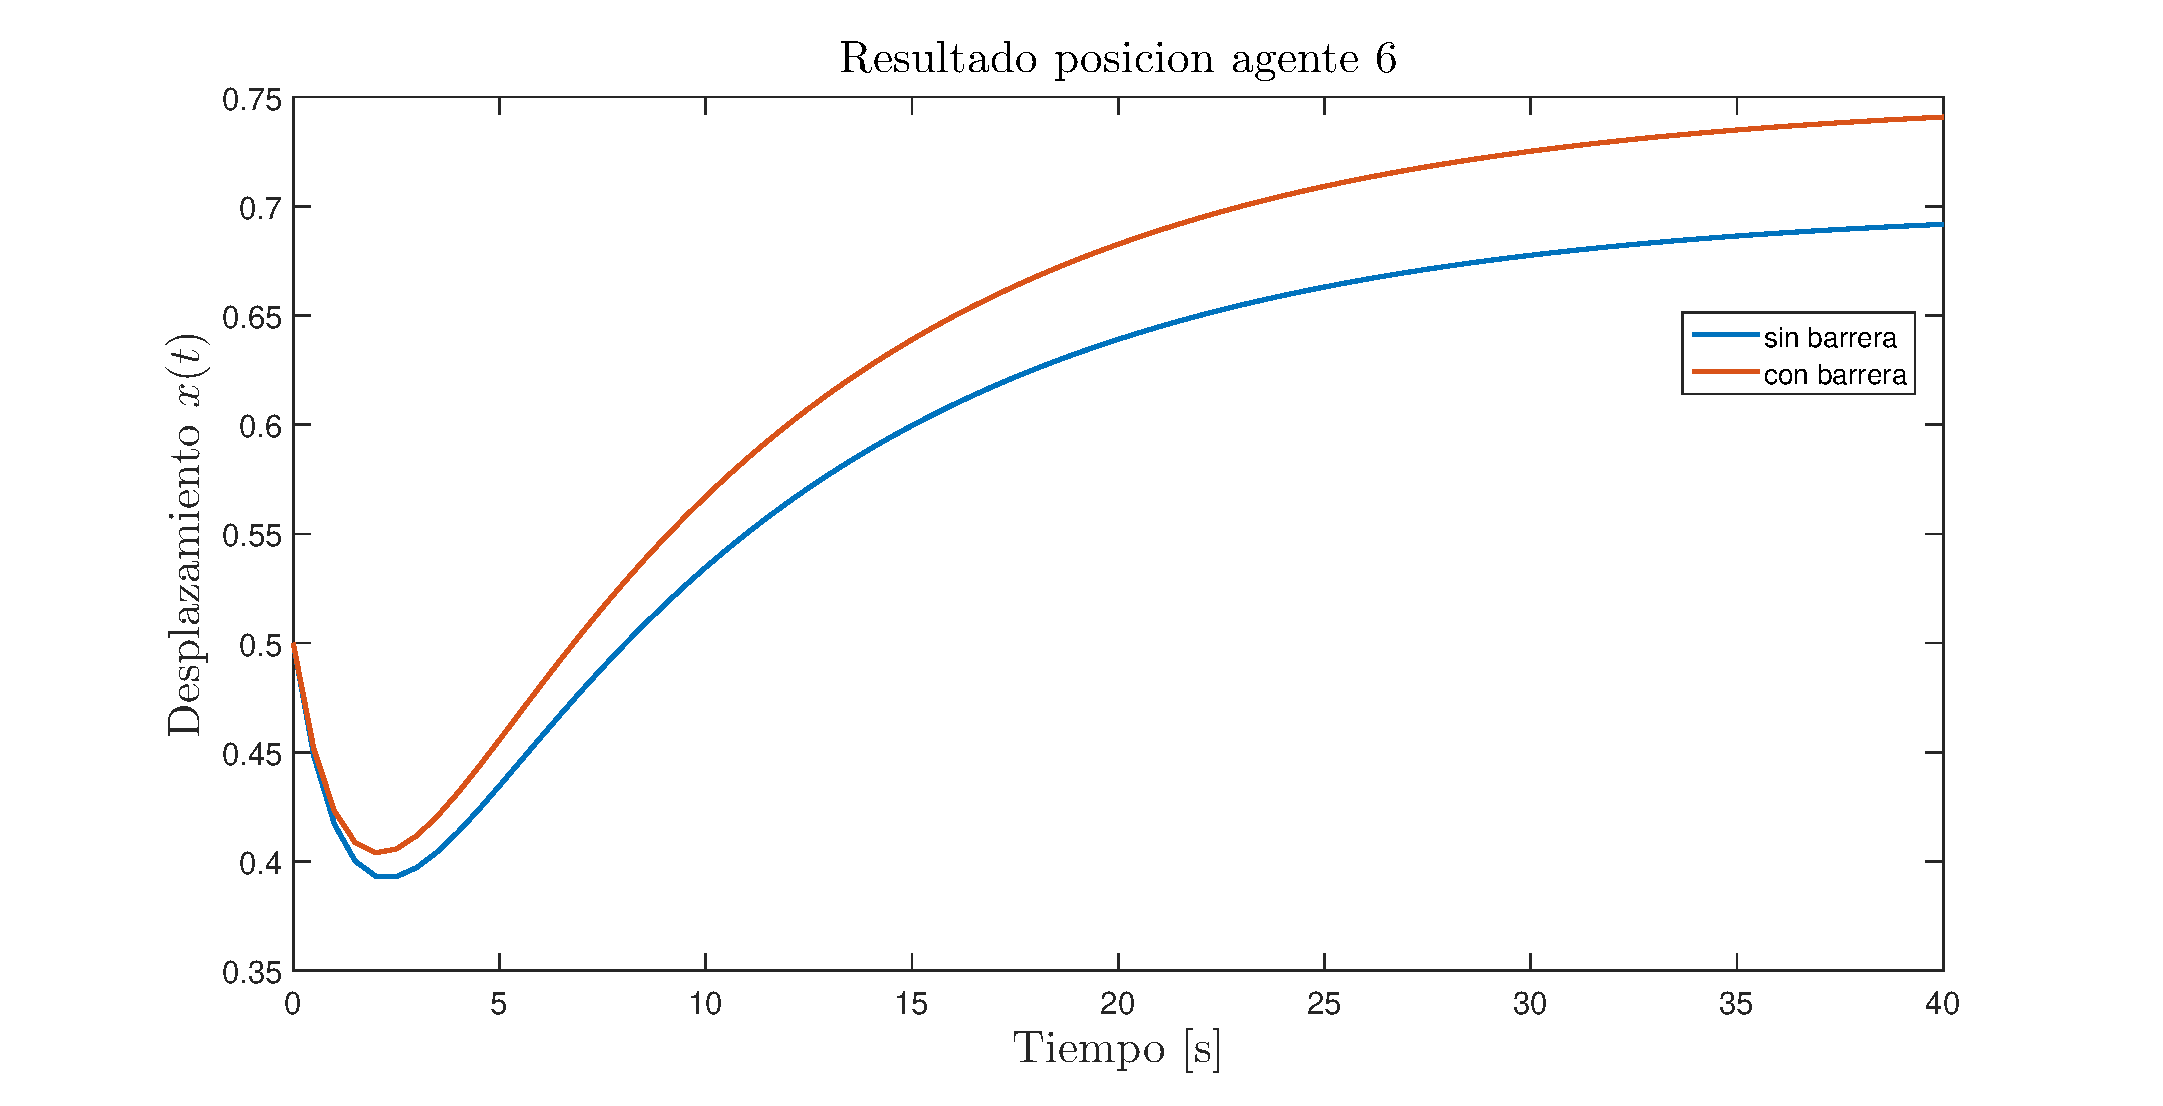
\includegraphics[width=3.9in]{imagenes/efecto_barrera.eps}
	\caption{Trayectoria del agente 6 con y sin barrera}
	\label{fig_efecto_barrera}
\end{figure}
En la Figura \ref{fig_efecto_barrera} se muestra e comportamiento de uno de los agentes con y sin la presencia de la restricción. Se evidencia que cunado la restricción está activa las dinámicas son más rápidas, y este efecto aumentará a medida que el sistema se acerque a los valores de la restricción.
